\documentclass[12pt]{article}
\pagenumbering{gobble}
\linespread{1}

\usepackage{amsfonts}
\usepackage{amsmath}
\usepackage{amssymb}
\usepackage{array}
\usepackage{fancyhdr}
\usepackage{textcomp}
\usepackage{pgfplots}
\usepackage[margin=1in,headheight=10mm]{geometry}

\usetikzlibrary{fillbetween}

\pgfplotsset{compat=1.17}

\newcommand{\contradiction}{%
    \ensuremath{{\Rightarrow\mspace{-2mu}\Leftarrow}}%
}

\newcommand{\angleb}[1]{\left\langle#1\right\rangle}
\newcommand{\vertb}[1]{\left\vert#1\right\vert}

\begin{document}
\pagestyle{fancy}
\fancyhead{}
\fancyhead[L]{Alexander Agruso}
\fancyhead[R]{Homework 1}

\normalsize
\section*{Exercises 12.1}
\begin{itemize}
    \item [5.)] In $\mathbb{R}^2$, $x=4$ represents a line, while in $\mathbb{R}^3$, $x=4$ represents a plane.

    \begin{tikzpicture}
        \begin{axis}[
            enlargelimits=false,
            grid=major,
            xmin=-6,xmax=6,
            ymin=-6,ymax=6,
            domain=-6:6,
            xtick={-3,0,3},
            ytick={-3,0,3},
            xlabel={$x$},
        ]
        \addplot[color=blue] table[row sep = crcr]{4 6 \\ 4 -6 \\};
        \end{axis}
    \end{tikzpicture}

    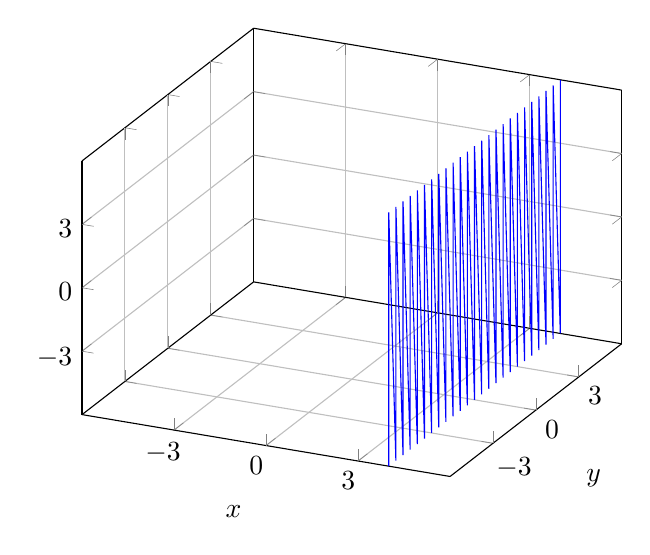
\begin{tikzpicture}
        \begin{axis}[
            enlargelimits=false,
            grid=major,
            xmin=-6,xmax=6,
            ymin=-6,ymax=6,
            zmin=-6,zmax=6,
            domain=-6:6,
            xtick={-3,0,3},
            ytick={-3,0,3},
            ztick={-3,0,3},
            xlabel={$x$},
            ylabel={$y$},
            ]
            \addplot3[color=blue](4,y,x);
        \end{axis}
    \end{tikzpicture}

    \item [7.)] $x+y=2$ represents a plane in $\mathbb{R}^3$:

    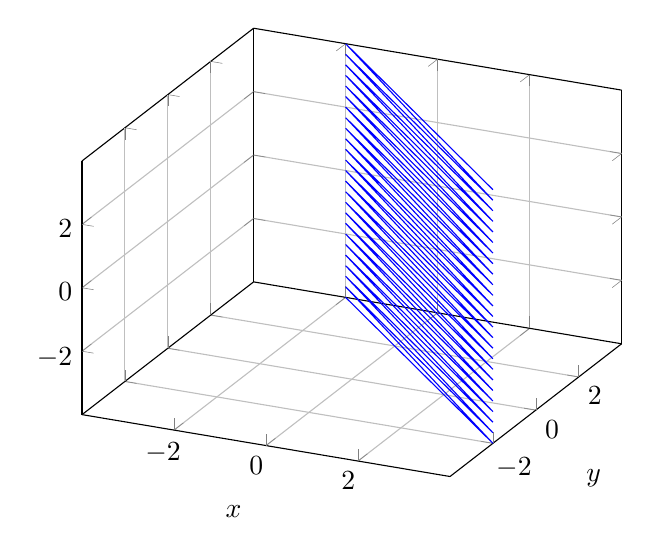
\begin{tikzpicture}
        \begin{axis}[
            enlargelimits=false,
            grid=major,
            xmin=-4,xmax=4,
            ymin=-4,ymax=4,
            zmin=-4,zmax=4,
            domain=-2:4,
            y domain=-4:4,
            xtick={-2,0,2},
            ytick={-2,0,2},
            ztick={-2,0,2},
            xlabel={$x$},
            ylabel={$y$},
            ]
            \addplot3[color=blue](x,2-x,y);
        \end{axis}
    \end{tikzpicture}

    \item [12.)] \begin{itemize}
        \item [c.)] $y=-2$, thus the distance between $(4,-2,6)$ and the $xz$-plane is $\vert y\vert=2$.

        \item [e.)] $x=4$ and $z=6$, thus the distance between $(4,-2,6)$ and the $y$-axis is $\Vert\angleb{x,y}\Vert=\sqrt{4^2+6^2}=\sqrt{16+36}=\sqrt{52}=2\sqrt{13}$.
    \end{itemize}

    \item [13.)] The equation for the sphere is $(x+3)^2+(y-2)^2+(z-5)^2=16$; setting $x=0$ for the intersection of the sphere and the $yz$-plane, we find it to be $(y-2)^2+(z-5)^2=16-9=7$, or a circle with center $(0,2,5)$ and radius $\sqrt{7}$.

    \item [15.)] The line segment between points $P(4,3,-1)$ and $Q(3,8,1)$ is a radius of the sphere, thus $\left\Vert{\Vec{p}-\Vec{q}}\right\Vert=\sqrt{(4-3)^2+(3-8)^2+(-1-1)^2}=\sqrt{1+25+4}=\sqrt{30}$ is the length of the radius, thus the equation for the sphere is $(x-3)^2+(y-8)^2+(z-1)^2=30$.

    \item [17.)] We can rearrange the equation as follows:
    \begin{align*}
        x^2+y^2+z^2-2x-4y+8z&=15\\
        (x^2-2x+1)+(y^2-4y+4)+(z^2+8z+16)&=15+1+4+16\\
        (x-1)^2+(y-2)^2+(z+4)^2=36=6^2
    \end{align*}
    Thus the equation represents a sphere with center $(1,2,-4)$ and radius 6.

    \item [27.)] $y<8$ represents all points behind the plane $y=8$.

    \item [29.)] $0\leq z\leq6$ represents all points on or between the planes $z=0$ and $z=6$.

    \item [35.)] $1\leq x^2+y^2+z^2\leq 5$ represents a spherical shell with an inner radius of 1 and an outer radius of $\sqrt{5}$.
\end{itemize}

\section*{Exercises 12.2}
\begin{itemize}
    \item [5.)] \begin{itemize}
        \item [a.)] $\vec{u}+\vec{v}$:

        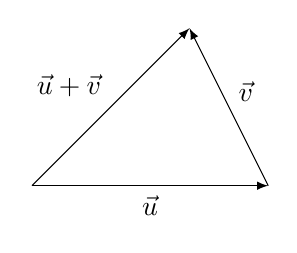
\begin{tikzpicture}
            \draw[-latex] (0,0) -- node[below] {$\vec{u}$} (3,0);
            \draw[-latex] (3,0) -- node[yshift=2mm,right] {$\vec{v}$} (2,2);
            \draw[-latex] (0,0) -- node[above left] {$\vec{u}+\vec{v}$} (2,2);
        \end{tikzpicture}

        \item [d.)] $\vec{u}-\vec{v}$:

        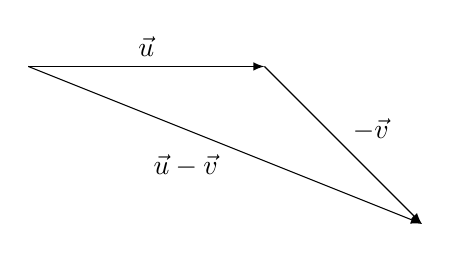
\begin{tikzpicture}
            \draw[-latex] (0,0) -- node[above] {$\vec{u}$} (3,0);
            \draw[-latex] (3,0) -- node[yshift=2mm,right] {$-\vec{v}$} (5,-2);
            \draw[-latex] (0,0) -- node[below,xshift=-5mm] {$\vec{u}-\vec{v}$} (5,-2);
        \end{tikzpicture}

        \pagebreak
        \item [f.)] $\vec{u}-\vec{w}-\vec{v}$:

        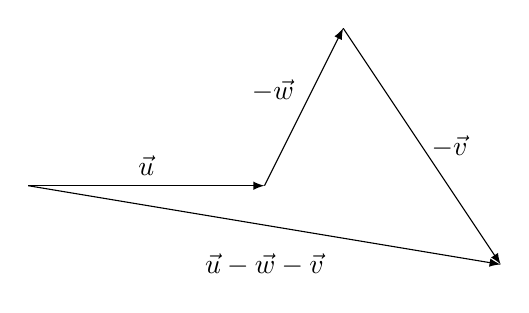
\begin{tikzpicture}
            \draw[-latex] (0,0) -- node[above] {$\vec{u}$} (3,0);
            \draw[-latex] (3,0) -- node[yshift=2mm,left] {$-\vec{w}$} (4,2);
            \draw[-latex] (4,2) -- node[right] {$-\vec{v}$} (6,-1);
            \draw[-latex] (0,0) -- node[yshift=-5mm] {$\vec{u}-\vec{w}-\vec{v}$} (6,-1);
        \end{tikzpicture}
    \end{itemize}

    \item [9.)] $B-A=\left\langle 1,2\right\rangle-\left\langle-2,1\right\rangle=\left\langle3,1\right\rangle$

    \begin{tikzpicture}
        \draw[-latex] (-3,0) -- (4,0) node[right] {$x$};
        \draw[-latex] (0,-1) -- (0,3) node[above] {$y$};
        \draw[-latex] (-2,1) node[yshift=4mm] {$A$} -- (1,2) node[above] {$B$};
        \draw[-latex] (0,0) -- (3,1) node[above] {$a$};
    \end{tikzpicture}

    \item [13.)] $B-A=\left\langle2,3,-1\right\rangle-\left\langle0,3,1\right\rangle=\left\langle2,0,-2\right\rangle$

    \begin{tikzpicture}
        \draw[-latex] (0,0,0) -- (2,0,0) node[right] {$x$};
        \draw[-latex] (0,0,0) -- (0,2,0) node[above] {$z$};
        \draw[-latex] (0,0,0) -- (0,0,2) node[below] {$y$};
        \draw[-latex] (0,0.5,1.5) node[above] {$A$} -- (1,-0.5,1.5) node[below] {$B$};
        \draw[-latex] (0,0,0) -- (1,-1,0) node[right] {$a$};
    \end{tikzpicture}

    \item [19.)] $a+b=\angleb{-3,4}+\angleb{9,-1}=\angleb{6,3}$\newline
    $4a+2b=4\angleb{-3,4}+2\angleb{9,-1}=\angleb{-12,16}+\angleb{18,-2}=\angleb{6,14}$\newline
    $\vertb{a}=\sqrt{(-3)^2+4^2}=\sqrt{9+16}=\sqrt{25}=5$\newline
    $\vertb{a-b}=\sqrt{(-12)^2+5^2}=\sqrt{144+25}=\sqrt{169}=13$

    \item [21.)] $a+b=4i-3j+2k+2i-4k=6i-3j-2k$\newline
    $4a+2b=4(4i-3j+2k)+2(2i-4k)=16i-12j+8k+4i-8k=20i-12j$\newline
    $\vertb{a}=\vertb{4i-3j+2k}=\sqrt{4^2+(-3)^2+2^2}=\sqrt{16+9+4}=\sqrt{29}$\newline
    $\vertb{a-b}=\vertb{2i-3j-6k}=\sqrt{2^2+(-3)^2+(-6)^2}=\sqrt{4+9+36}=\sqrt{49}=7$

    \pagebreak
    \item [25.)] Let $\vec{v}=8i-j+4k$. We can find the unit vector of $\vec{v}$ by evaluating $\frac{\vec{v}}{\Vert\vec{v}\Vert}$.
    \begin{equation*}
        \Vert\vec{v}\Vert=\sqrt{8^2+(-1)^2+4^k}=\sqrt{64+1+16}=\sqrt{81}=9
    \end{equation*}
    \begin{equation*}
        \frac{\vec{v}}{\Vert\vec{v}\Vert}=\frac{1}{9}\vec{v}=\frac{8}{9}i-\frac{1}{9}j+\frac{4}{9}k
    \end{equation*}
    Which is the unit vector of $\vec{v}$.

    \item [31.)] $x=r\cos\theta=60\cos(40^\circ)\approx45.96$\newline
    $y=r\sin\theta=60\sin(40^\circ)\approx38.57$
\end{itemize}

\section*{Exercises 12.3}
\begin{itemize}
    \item [3.)] $a\cdot b=[1.5(-4)+0.4(6)]=-6+2.4=-3.6$

    \item [7.)] $a\cdot b=[2(1)+1(-1)+0(1)]=2-1+0=1$

    \item [9.)] $a\cdot b=\Vert a\Vert\Vert b\Vert\cos\theta=(7)(4)\cos(30^\circ)=28\frac{\sqrt{3}}{2}=14\sqrt{3}$

    \item [19.)] $\Vert a\Vert=\sqrt{4^2+(-3)^2+1^2}=\sqrt{16+9+1}=\sqrt{26}$\newline
    $\Vert b\Vert=\sqrt{2^2+0^2+(-1)^2}=\sqrt{4+1}=\sqrt{5}$\newline
    $a\cdot b=[4(2)-3(0)+1(-1)]=(8-1)=7$\newline
    $\frac{a\cdot b}{\Vert a\Vert\Vert b\Vert}=\frac{7}{\sqrt{130}}$\newline
    $\theta=\cos^{-1}(\frac{7}{\sqrt{130}})\approx52.13^\circ$

    \item [27.)] Let $\vec{v}=\angleb{x,y,z}$. For $\vec{v}$ to be orthogonal to both $i+j$ and $i+k$, $\vec{v}\cdot\angleb{1,1,0}=\vec{v}\cdot\angleb{1,0,1}=0$, thus $x+y=x+z=0$. Let $\vec{v}=\angleb{1,-1,-1}$, thus $\vec{v}\cdot\angleb{1,1,0}=[1(1)-1(1)-1(0)]=1-1=0$, and $\vec{v}\cdot\angleb{1,0,1}=[1(1)-1(0)-1(1)]=1-1=0$, thus $\vec{v}$ is orthogonal to both vectors. To find the unit vector of $\vec{v}$, evaluate $\frac{\vec{v}}{\Vert v\Vert}=\frac{\vec{v}}{\sqrt{3}}=\angleb{\frac{1}{\sqrt{3}},-\frac{1}{\sqrt{3}},-\frac{1}{\sqrt{3}}}$.

    \item [29.)] $2x-y=3\implies y=2x-3$, thus $\angleb{1,2}$ represents this equation.\newline
    $3x+y=7\implies y=7-3x$, thus $\angleb{1,-3}$ represents this equation.\newline
    $\Vert\angleb{1,2}\Vert=\sqrt{1^2+2^2}=\sqrt{5}$, $\Vert\angleb{1,-3}\Vert=\sqrt{1^2+(-3)^2}=\sqrt{10}$\newline
    $\angleb{1,2}\cdot\angleb{1,-3}=(1(1)+2(-3))=1-6=-5$\newline
    $\theta=\cos^{-1}\left(\frac{-5}{\sqrt{5}\sqrt{10}}\right)=135^\circ$, thus the acute angle is $45^\circ$.
\end{itemize}

\end{document}
